\section{Experiment 1: theoretical simulation}
As we've seen before, the loudspeaker array in the laboratory can be modelled as an octagon of monopoles (\autoref{WFSdistribution}). If a monopole source is placed outside the area, the loudspeaker array should be able to replicate the field with opposite sign and hence, cancel it inside the octagon. As explained in \autoref{optimization}, the election of points matters when applying the global scalation of loudspeaker coefficients (\autoref{OptScalation}). Therefore, a more or less even distribution of points should be chosen.

As an example, \autoref{figTheoCanc} shows the result for a noise source at position $[-1, 2.5, 0]$, and the optimization applied for the points represented by microphone icons.

\begin{figure}
	\centering
	\reflectbox{\rotatebox[origin=c]{180}{
			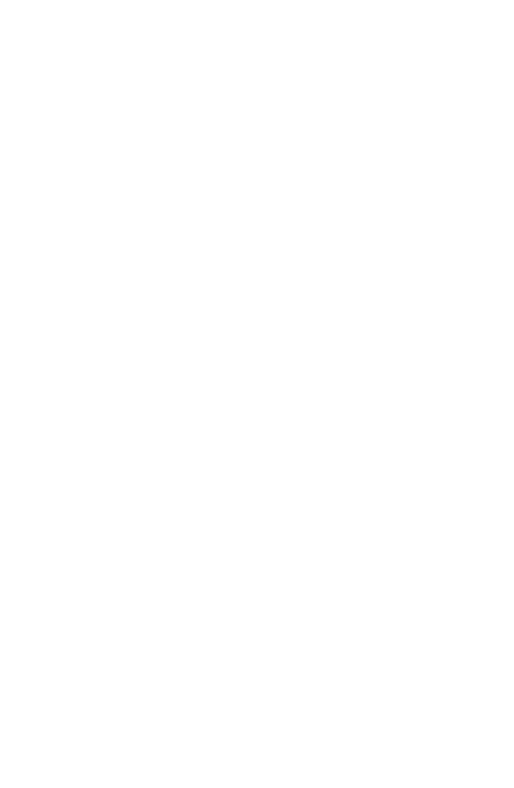
\includegraphics[height=0.3\textheight]{./Img/Experiment1_Example.pdf}
	}}	
	\caption[WFS cancellation]{WFS cancellation. $\rns = [-1, 2.5, 0]$.}
	\label{figTheoCanc}
\end{figure}


\section{Experiment 2: GTAC acoustic paths}
The first experiment is a completely theoretical one, although it uses results from previous measures. The acoustic responses in the GTAC laboratory for different points was measured with high precision previously, and the results are published in the website. In total, the measures were done in 360 points distributed in a rectangular grid of size $24$x$15$ and separation of $20 \si{cm}$ between adjacent nodes (\autoref{GTAC360micro}).

\begin{figure}
	\centering
	\reflectbox{\rotatebox[origin=c]{180}{
			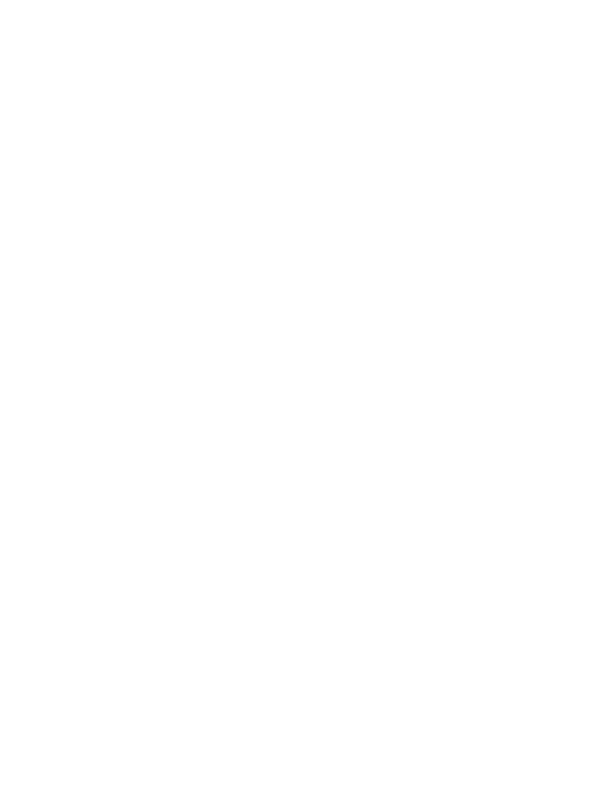
\includegraphics[height=0.3\textheight]{./Img/WFSGTAC360microphones.pdf}
	}}	
	\caption[Schematic of measures in GTAC anechoic chamber]{Schematic of measures in GTAC anechoic chamber}
	\label{GTAC360micro}
\end{figure}

%We could apply the optimization already described in \autoref{optimization}, but there is a problem. GTAC responses are measured for loudspeakers in the WFS array, but of course, not for loudspeakers outside the array in arbitrary positions. Hence, we can only guess the acoustic paths by applying the theoretical model (\autoref{acPathTheoric}), in which case we assume that the noise source is isotropic. Then, we apply the optimization process and see how far we can go in the cancellation. Only the first type of optimization is interesting since the position of the noise loudspeaker is known.

GTAC responses are measured for loudspeakers in the WFS array, but of course, not for loudspeakers outside the array in arbitrary positions. Hence, we can only guess the acoustic paths by applying the theoretical model (\autoref{acPathTheoric}), in which case we assume that the noise source is isotropic.

Results are shown in \reffig{}. Different positions have been used. As we can see, cancellations of X dB are easy to achieve.



\section{Experiment 3: lab recording}
